\usemintedstyle{tango}
\setminted[python]{fontsize=\footnotesize, breaklines}
In the first part of this thesis we have established a theoretical basis about multigrid methods, formal languages and genetic programming.
In Chapter~\ref{chapter:multigrid-formal-language}, building on this foundation, we have then developed a novel formal language and grammar for the automatic generation of multigrid methods. 
While we have already demonstrated that the capabilities of this approach in alternating each individual step of a multigrid method, we could not yet prove its benefits compared to the use of classical multigrid cycles, such as V-, F- and W-cycles.
We aim to achieve this goal with the implementation of \emph{EvoStencils}, a prototypical Python framework for the grammar-guided optimization of multigrid methods.
Using this framework we will then show how it is possible to evolve methods that are more efficient than all common multigrid cycles in solving a number of PDE-based problems while being structurally different that any other known method of this type.
However, before we discuss EvoStencils' features and their implementation in Python, we want to provide an overview about its workflow and software architecture.
In general, we can distinguish between EvoStencils' core implementation and the functionality of the framework that is build upon the use of external libraries.
First of all, since our formulation of the rules to construct a multigrid methods in the form of a context-free grammar, we can utilize the grammar-guided genetic programming techniques presented Chapter~\ref{chapter:formal-languages-and-gp} without adapting their inner workings.
For this purpose, we employ the widely-used evolutionary computation framework DEAP\footnote{DEAP: \url{https://github.com/deap/deap}}~\cite{rainville2012deap}, which enables us to implement GGGP in a modular way while requiring only a limited amount of adaption.
However, the questions that then remains to be answered how we can evaluate each multigrid method obtained through GGGP in an automatic and reproducible manner.
As we have seen in Section~\ref{sec:grammar-based-algorithm-generation} the 
application of the sequence of state transition functions represented in a given derivation tree produces a computational graph of the form of Figure~\ref{fig:example-three-grid-method-computational-graph}, which can then be transformed to an algorithmic representation, as shown in Algorithm~\ref{alg:example-three-grid-method-generated}.
However, while any expert could now manually implement the corresponding multigrid solver based on this representation using an arbitrary numerical software package, within GGGP we have to evaluate each method in an automatic way without requiring any human intervention.
Recently, code-generation techniques based on the specification of a numerical solver in a high-level domain specific language (DSL) have become increasingly powerful~\cite{kostler2020code}.
An example for this approach is the ExaStencils framework~\cite{lengauer2020exastencils,lengauer2014exastencils}, which has been specifically designed for the automatic generation of fast and scalable implementation of multigrid-based solvers specified in a tailored DSL called ExaSlang~\cite{schmitt2014exaslang,schmitt2016systems,kuckuk2016automatic}.
ExaSlang enables the formulation of a multigrid method as a sequence of high-level operations, without the need to consider the implementation details of each individual statement, while still granting the user the flexibility to apply further optimizations through the addition of code transformations and lower-level statements.
To evaluate a given solver, obtained from a grammar-based representation, we, therefore, emit its corresponding algorithmic formulation as an ExaSlang specification, based on which we then employ the ExaStencils framework to generate a scalable C++ implementation.
The resulting program can then be executed on a number of test cases in order to measure the desired performance characteristics of the solver.
Finally, note that the execution of a GGGP-based optimization approach requires the evaluation of a large number of different multigrid methods.
Depending on the problem that one aims to solve it can be infeasible to perform the optimization on a single compute node, necessitating the implementation of a multi-node parallelization.
The message passing interface (MPI)~\cite{walker1996mpi} provides a unified interface for performing parallel computations on a distributed system that is supported by the majority of supercomputing devices available.
While MPI has been originally designed for the traditional scientific computing languages Fortran and C, it recently has been also made available within Python~\cite{dalcin2021mpi4py}. 
With the addition of MPI, as a distributed computing backend, we arrive at the following high-level view of EvoStencils' software architecture, which is shown in Figure~\ref{fig:evostencils-architecture}.
\begin{figure}
	\resizebox{\columnwidth}{!}{%
		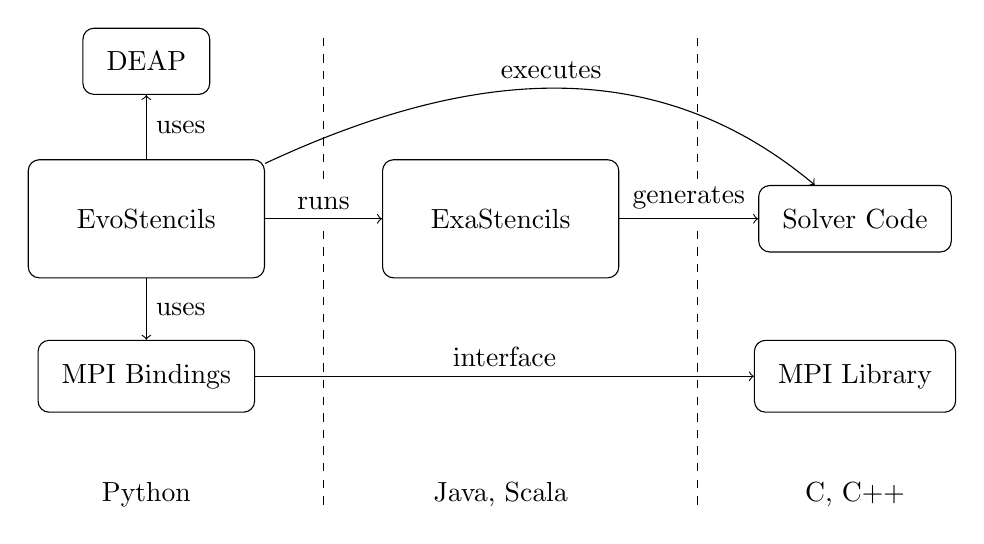
\begin{tikzpicture}
			%\draw [help lines] (-10,-10) grid (10,10);
			\node[draw, minimum width=3cm, minimum height=1.5cm, rounded corners] (evo) at (0,0) {EvoStencils};
			\node[draw, inner sep=3mm, rounded corners] (bindings) at (0, -2) {MPI Bindings};
			\node[draw, inner sep=3mm, rounded corners] (deap) at (0, 2) {DEAP};
			\node[draw, minimum width=3cm, minimum height=1.5cm, rounded corners] (exa) at (4.5, 0) {ExaStencils};
			\node[draw, inner sep=3mm, rounded corners] (code) at (9, 0) {Solver Code};
			\node[draw, inner sep=3mm, rounded corners] (mpi) at (9, -2) {MPI Library};
			\draw[dashed] (2.25, 2.3) -- (2.25,0.5);
			\draw[dashed] (2.25, -0.15) -- (2.25,-3.7);
			\draw[dashed] (7, 2.3) -- (7,0.5);
			\draw[dashed] (7, -0.15) -- (7,-3.7);
			\node (python) at (0, -3.5) {Python};
			\node (java) at (4.5, -3.5) {Java, Scala};
			\node (c) at (9, -3.5) {C, C++};
			\draw[->] (evo)-- node[anchor=west] {uses} (deap);
			\draw[->] (evo)-- node[anchor=south]{runs} (exa);
			\draw[->] (exa)--node[anchor=south] {generates} (code);
			\draw[->] (evo) to [out=25,in=140] node[anchor=south] {executes} (code);
			\draw[->] (bindings)--node[anchor=south] {interface}(mpi);
			\draw[->] (evo)--node[anchor=west] {uses}(bindings);
			%\draw[->] (mpi)--(code);
		\end{tikzpicture}
	}\caption{Software Architecture of EvoStencils.}
	\label{fig:evostencils-architecture}
\end{figure}
In the following, we will now consider the individual parts of this architecture in more detail, starting with the core implementation of EvoStencils, which can be considered as a separate module that does not depend on any of the other tools and libraries mentioned here.
As a first step, we will outline the implementation of an intermediate representation for multigrid methods that can be easily obtained from a given derivation tree and which then acts as a basis for all subsequent steps of solver generation and evaluation.

\section{Intermediate Representation}
\label{sec:intermediate-representation}
Before we can represent the actual method and its computational structure, we need to be aware of the fact that all operations of a multigrid method are defined on a grid with certain step size.
Note that algebraic multigrid methods~\cite{stuben2001introduction,ruge1987algebraic}, which are not considered in this work, represent an exception to this, as they directly operate on sparse matrix and vector data structures.
In Section~\ref{sec:discretization} we have already made the assumption that we are able to discretize the underlying PDE on a hierarchy of structured grids.
Therefore, to identify a grid within this hierarchy certain information is required, which we store in a \emph{Grid} data structure whose implementation is shown in Listing~\ref{code:ir:grid}.
In general a structured grid is identified by its size, i.e. the number of grid points, and spacing $h$ in each dimension.
In addition we also include the grid's level to identify it within the discretization hierarchy.
Note that in case the grid is uniform we only need to store a single value for the spacing in each dimension, while otherwise a value needs to be stored for each pair of grid points.
As the problems considered in this work are all solved on a hierarchy of uniform grids, we focus on this particular case.
However, whenever we apply this restriction it is clearly stated within the respective part of the code.  
\begin{listing}
	\inputminted{python}{evostencils/ir/grid.py}
	\caption{IR: Structure Grid}
	\label{code:ir:grid}
\end{listing}
After defining a data structure that provides all information about a certain grid within the discretization hierarchy, we can start defining expressions that operate on this data structure.
For this purpose, first in Listing~\ref{code:ir:abstact-base-class} a common abstract base class is provided from which all subsequent expression classes are derived.
\begin{listing}
	\inputminted{python}{evostencils/ir/expression.py}
	\caption{IR: Abstract Expression Base Class}
	\label{code:ir:abstact-base-class}
\end{listing}
In addition to the already mentioned grid data structure this class also defines a \emph{shape} for each expression.
From a mathematical point of view, each expression contained in a multigrid method either computes a matrix or a vector, whose shape can be derived recursively from its operands
The shape of the corresponding expression is then defined as a pair $(r, c)$, whose first entry $r$ corresponds to the number of rows and the second $c$ to the number of columns, which in the given example is both $m$.
Based on this abstract class, we can then further distinguish between predefined entities, such as the system matrix and right-hand side, and expressions that refer to the mathematical operations of a multigrid method.
First of all, Listing~\ref{code:ir:entity} contains the implementation of the entity base class.
\begin{listing}
	\inputminted{python}{evostencils/ir/entity.py}
	\caption{IR: Entity Base Class}
	\label{code:ir:entity}
\end{listing}
In addition to the previously mentioned attributes, this class is also given a \emph{name} to identify the respective entity.
Based on this implementation we can then further define classes for representing an approximate solution and right-hand side and operator, which are shown in the Listings~\ref{code:ir:approximation} and~\ref{code:ir:operator}.
\begin{listing}
	\inputminted{python}{evostencils/ir/approximation.py}
	\caption{IR: Approximate Solution and Right-Hand Side}
	\label{code:ir:approximation}
\end{listing}
\begin{listing}
	\inputminted{python}{evostencils/ir/operator.py}
	\caption{IR: Operator}
	\label{code:ir:operator}
\end{listing}
In both cases, the shape of the respective entity is obtained by computing the grid size product over all dimensions, whereas in case of the approximation and right-hand side the result can be considered as a vector while the shape of an operator corresponds to a quadratic matrix.
Note that as the \emph{Approximation} and \emph{RightHandSide} classes, from a mathematical point of view, can be both considered as a vector, we only implement the former and then utilize inheritance to avoid unnecessary code duplication.
In addition to the attributes defined in its parent class, the \emph{Approximation} includes a \emph{predecessor} attribute, whose meaning will be discussed later within the implementation of grammar generation.
While the other two entities discussed here correspond to the solution and right-hand side of a discretized PDE, Listing~\ref{code:ir:operator} represents its operator, given in form of one or multiple stencil codes.
In Section~\ref{subsec:stencil-codes} we have already introduced a mathematical notation for stencil codes in form of Equation~\ref{eq:stencil-definition}, which can be implemented in the Python programming language in a straightforward manner that leads to the \emph{Stencil} class shown in Listing~\ref{code:ir:stencil}.
%TODO introduce stencil implementation here
\begin{listing}
	\inputminted{python}{evostencils/ir/stencil.py}
	\caption{IR: Stencil}
	\label{code:ir:stencil}
\end{listing}
The \emph{entries} attribute of this class directly corresponds to the set $S_h$ defined in Equation~\ref{eq:stencil-definition}, whereby we use a \emph{tuple} object to represent this set in the Python programming language.
Each entry $e_i$ of this tuple then again represents a tuple of the form of
\begin{equation}
	e_i = \left(\bm{a}_i, b_i \right),
\end{equation} 
where $\bm{a}_i$ is the offset from the current grid point in each dimension, given as an array of integer values, and $b_i$ is the stencil value that corresponds to each offset, given as a floating point number.
Based on this class we can then provide implementations for all operations on stencil codes that have been defined in Section~\ref{subsec:stencil-codes}.
Furthermore, in accordance with Section~\ref{subsec:systems-of-pdes} and~\ref{subsec:block-smoothing}, we can extend this implementation to systems of PDEs and block smoothers, which will be briefly covered in the next Chapter of this thesis. %TODO insert ref to next chapter here or remove sentence
Now note that in our implementation of the \emph{Operator} class in Listing~\ref{code:ir:operator} the stencil is not included directly, but instead we provide a so-called \emph{stencil generator}.
A stencil generator is a function that returns the discretization of an operator on a particular grid in the form of a stencil.
For instance, the finite-difference discretization of the Laplace operator $\nabla^2$ on a two-dimensional uniform grid leads to the stencil 
\begin{equation*}
	\begin{split}
		\Delta_{h,h} = & \; \big\{ \left( \left( 0,0 \right), 4 / h^2 \right), \left(\left(1,0\right), -1/h^2\right), \left(\left(-1,0\right), -1 / h^2\right), \\ & \left(\left(0,1\right), -1/h^2\right), \left(\left(0,-1\right), -1/h^2\right) \big\}_{h,h}.
	\end{split}
\end{equation*}
in which the value at each offset depends on the grid spacing $h$.
Furthermore, in certain cases it is possible to construct the higher-dimensional version of a stencil from its lower dimensional counterparts, as we have shown in Section~\ref{subsec:restriction-and-prolongation} for the considered prolongation and restriction operators.
Therefore, instead of storing a unique stencil for each individual operator instance, we can instead parametrize its generation based on the features of the applied discretization, by including a reference to the respective generator function.
Finally, as both prolongation and restriction transfer information between adjacent grids within a hierarchy of discretizations, they can be considered as a special case of an operator, which, for instance, leads to a different value of the \emph{shape} attribute.
For this purpose, the class \emph{InterGridOperator}, from which all restriction and prolongation operators are derived, extends the \emph{Operator} class with the required functionality.
For the sake of brevity, the implementation of this class and the respective \emph{Restriction} and \emph{Prolongation} subclasses can be found in the appendix.

After discussing the implementation of the different entities based on which a multigrid method is built, we next shift our attention to the implementation of those IR classes that let us represent the expressions that correspond to the actual computations performed within its application. 
For this purpose we, first provide general classes for representing unary and binary expressions, which are shown in the Listings~\ref{code:ir:unary-expression} and~\ref{code:ir:binary-expression}.
\begin{listing}
	\inputminted{python}{evostencils/ir/unary_expression.py}
	\caption{IR: Unary Expression Base Class}
	\label{code:ir:unary-expression}
\end{listing}
\begin{listing}
	\inputminted{python}{evostencils/ir/binary_expression.py}
	\caption{IR: Binary Expressions Base Class}
	\label{code:ir:binary-expression}
\end{listing}
In both cases, all necessary properties are obtained from the expression's operands in a recursive manner.
However, as in case of a binary expression the shape of the result depends on the type of operation, we raise an error if this method is not implemented in one of the derived classes. 
While we will later see that there exist certain expressions that do not fall into these categories the majority of multigrid operations can be already expressed based on these two classes.
Again we have included a number of specific examples in the appendix.
As it has been discussed in Section~\ref{sec:grammar-based-algorithm-generation}, we aim to represent the computational structure of a given multigrid method in form of a redundancy-free directed graph. 
While the previously defined base classes allow us to represent the arithmetic expressions that occur within the correction terms of a multigrid method, there are two operations that require a special treatment.
As we have already seen in Figure~\ref{fig:example-three-grid-method-computational-graph} it is necessary to access previously computed intermediate results at multiple occasions within a multigrid method.
In particular, each time a coarse-grid correction is performed we have to restore the previous approximate solution and right-hand side on the respective level.
Furthermore, whenever we compute a new residual the current expression for both the right-hand side as well as the approximate solution are required.
For this purpose, we implement the classes \emph{Residual} and \emph{Cycle}, which serve the special-purpose of including additional references to previously defined expressions within a multigrid method.
Each of these references then corresponds to one of the subgraphs in Figure~\ref{fig:example-three-grid-method-computational-graph} whose root node possesses multiple incoming edges, i.e. the ones that have been annotated in Figure~\ref{fig:example-three-grid-method-computational-graph-annotated}.
We will later see how to utilize these references in order to construct a complete graph from the grammar-based representation of a multigrid method.
Listing~\ref{code:ir:residual} shows the implementation of the \emph{Residual} class, which contains references to the system operator $A_H$, the expression for computing the current approximate solution $\tilde{x}_H$ and right-hand side $b_H$, where $H$ is the grid spacing on the current level.
Based on these components we can, thus, easily construct the corresponding residual expression $b_H - A_H \tilde{x}_H$.
\begin{listing}
	\inputminted{python}{evostencils/ir/residual.py}
	\caption{IR: Residual}
	\label{code:ir:residual}
\end{listing}
As a final step in the implementation of our intermediate representation, the definition of the \emph{Cycle} class is shown in Listing~\ref{code:ir:cycle}.
\begin{listing}
	\inputminted{python}{evostencils/ir/cycle.py}
	\caption{IR: Multigrid Cycle}
	\label{code:ir:cycle}
\end{listing}
This class implements the functionality to represent a single step of multigrid cycle on a certain level with spacing $H$ with the purpose to compute a new value for the approximate solution $\tilde{x}_H$, i.e.
\begin{equation}
	\tilde{x}_H = \tilde{x}_H + \omega c_H \; \text{with} \; P,
\end{equation}
where $c_H$ is a correction term, $\omega$ the relaxation factor and $P$ a partitioning.
Furthermore, to make the right-hand side available to subsequent steps of the method, such as for the computation of the residual, we, again, need to include an additional reference into the data structure.
Finally, we also include a reference to the previous state on the next finer level, such that in case the result of a cycle is applied a coarse-grid correction, the previous expression for the approximate solution and right-hand side can be restored on that level.
To better understand the purpose of these two classes consider the following example shown in Listing~\ref{code:ir:example.py}, which demonstrate the construction of a computational graph based on the intermediate representation introduced in this section.
\begin{listing}
	\inputminted{python}{evostencils/ir/example.py}
	\caption{Example Usage of the Intermediate Representation}
	\label{code:ir:example.py}
\end{listing}
Starting on the original problem on the finest level, we first store references to the initial approximate solution and right-hand side in an \emph{Cycle} object, which itself is included as a \emph{predecessor} reference into the subsequently created coarse-grid \emph{Cycle} object.
Finally, in order to apply the latter in form of a coarse-grid correction on the finest level, the original fine-grid \emph{Cycle} object is restored and its \emph{correction} variable is replaced by the respective expression which is obtained by prolongating the previously computed approximation on the coarse grid.
As this example demonstrate our intermediate representation (IR) enables us to construct the computational graph of a multigrid method in an iterative manner.
The next step towards the automatic generation of a multigrid method based on a grammar-based representation, now is to translate a sequence of derivations into the corresponding IR object.
For this purpose, we first have to consider how we can implement the formal system introduced in Section~\ref{sec:multigrid-grammar} using the functionality of the evolutionary computation framework DEAP~\cite{rainville2012deap}.
However, before we proceed with this discussion, we want to address some final remarks about the IR presented in this section.
First of all, note that while the main purpose of the implementation presented here is to uniquely represent the computational pattern of a multigrid method in form of a redundancy-free directed graph, in order to be able to construct this graph in a step-wise manner we have to include additional references into the respective nodes.
As we have shown in the previous discussion, the \emph{Cycle} class serves this purpose by including additional information about the current state of a multigrid method, according to Definition~\ref{def:multigrid-state}, in form of references to the current approximate solution and right-hand side.
While this information is important for the construction of the graph, it could be later discarded by replacing each \emph{Cycle} node with the respective arithmetic expression for computing an updated approximate solution, as it is shown in the \textsc{update} function in Section~\ref{sec:multigrid-state-transitions}.
However, preserving these additional references has the advantage of being able to easily traverse the sequence of \emph{Cycle} nodes within each graph.
This does not only enable us to quickly grasp the computational structure of the corresponding multigrid method, but also facilitates the identification of potential errors in the implementation.
We, therefore, represent each newly computed approximate solution by an \emph{Cycle} object, which is then referenced at each place of occurrence within subsequent computational steps of the method.
Also, note that even though the transformation of a graph-based to an algorithmic representation later requires us to translate each of these objects in a computational statement for updating the approximate solution, this operation can be performed while traversing the graph and, thus, does not induce a significant overhead within the process of algorithm generation. 
\section{Grammar Generation}
According to Section~\ref{sec:multigrid-grammar} our family of context-free grammar for the generation of multigrid methods consists of three components, a set of terminals, variables and productions, while additionally we have to choose a starting symbol $\ps{S}$ from the set of variables.
Furthermore, in Table~\ref{table:grammar-semantics} we have defined the semantics of each state transition function occurring within the productions listed in Table~\ref{table:multigrid-grammar}.
While Table~\ref{table:multigrid-grammar} fixes the number of coarsening steps, we have already seen that it is possible to define a similar grammar formulated on a different hierarchy of grid, for instance with a higher or lower number of coarsening steps.
We can, therefore, utilize this property to parametrize the generation of a grammar formulated on a particular hierarchy of grids with the employed number of coarsening steps.
For this purpose, we first need to generate the set of terminals that is defined on each level of the hierarchy, which is encapsulated into the class \emph{Terminals} shown in Listing~\ref{code:grammar:terminals}.
\begin{listing}
	\inputminted{python}{evostencils/grammar/terminals.py}
	\caption{Terminals defined on each level.}
	\label{code:grammar:terminals}
\end{listing}
Note that this class comprises a few notable differences compared to our grammar formulation in Section~\ref{sec:multigrid-grammar}.
First of all, as, at least in the applications considered in this work, each smoother is derived directly from the system operator, it does not need to be provided explicitly, but instead can be generated automatically within the grammar.
Also, while so far we have abstractly represented the application of the coarse-grid solver in form of a multiplication with the inverse $A^{-1}_H$ on the coarsest level with spacing $H$, the coarse-grid solver itself can also be considered as a degree of freedom, to be provided by the user.
The implementation of this class can again be found in the appendix.
Note that the coarse-grid solver may additionally contain an expression, again given in form of an IR object representing a multigrid method.
This enables the construction of multigrid methods in a hierarchical manner, which means that after obtaining a multigrid method on a certain hierarchy of discretizations, we can employ it as a coarse-grid solver for those methods whose coarsest grid corresponds to its topmost level.

\subsubsection{State Transition Functions}
\label{sec:evostencils:state-transition-functions}
As a next step, based on the \emph{Terminals} class, we can then implement the state transition functions that have been formulated in Section~\ref{sec:multigrid-state-transitions}, to construct the corresponding IR object of a multigrid method represented as a derivation tree of the grammar shown in Table~\ref{table:multigrid-grammar}.
From these components we will then finally be able assemble the actual grammar using the genetic programming module of the DEAP framework~\footnote{\url{https://deap.readthedocs.io/en/master/api/gp.html}}.
Listing~\ref{code:grammar:basic-functions} contains the implementation of each of the five state transition functions defined in Table~\ref{table:grammar-semantics}.
\begin{listing}
	\inputminted{python}{evostencils/grammar/base.py}
	\caption{State Transition: Basic Functions}
	\label{code:grammar:basic-functions}
\end{listing}
While the implementation of these function is semantically equivalent to their original definition, it comprises a number of differences that originate from the properties of the \emph{Cycle} class, shown in Listing~\ref{code:ir:cycle}.
In Section~\ref{sec:intermediate-representation} we have already discussed the advantages of representing the current state of a multigrid method directly within each \emph{Cycle} object.
As a consequence, the application of each state transition function either alters a given \emph{Cycle} or returns a new object of this type.
However, the \emph{residual} function deviates from this statement as it expects a \emph{state} variable as its argument, which corresponds to tuple, consisting of an approximation and right-hand side object.
The necessity of this modification can be understood by considering the grammar productions shown in Table~\ref{table:multigrid-grammar}.
While within each subsequent step of a multigrid method, each approximate solution is represented by a \emph{Cycle} objects that incorporates all steps required to compute its value, at the beginning of a multigrid method, the residual is computed based on the initial approximate solution $x_h^0$ and right-hand side $b_h$, given in the form of an \emph{Approximation} and \emph{RightHandSide} object, respectively.
In this case, we, therefore, need to pass the initial state 
\begin{equation*}
	S_h^0 = (x_h^0, b_h, \lambda, \lambda)
\end{equation*} explicitly to the respective residual function.
As the third and fourth entry of this tuple is empty, in Python this corresponds to a binary tuple consisting of the respective \emph{Approximation} and \emph{RightHandSide} object.
Even though in all subsequent computations, the first entry of this tuple consists of a \emph{Cycle} object, for the sake of simplicity, we simply include the right-hand side already included in this object as a second tuple entry, which enables us to utilize the same \emph{residual} function within all grammar productions.
For this purpose, we need to adapt the \emph{update} function accordingly, such that the respective binary state tuple, in the form of a \emph{Cycle} object, which computes a new approximate solution, and the current right-hand side, is returned.
Finally, as the last argument of the\emph{coarse\_grid\_correction} function result of an application of the \emph{update} function, it needs to be treated in a similar way.

The second main difference in the implementation shown in Listing~\ref{code:grammar:basic-functions} compared to our original definition of the \textsc{update} function is the representation of the relaxation factor as an index within a uniformly-sampled interval, which is included in the respective \emph{Terminal} object.
While we instead could explicitly store the relaxation factor as a floating point number, its representation accuracy then depends on the underlying floating point format.
Now assume we want to encode a certain derivation tree in a string-based format, which then later needs to be decoded in a different environment to restore the original information.
In case, each relaxation factor is stored as a floating point number, we need to ensure that each of these numbers is represented with the same accuracy in both environments.
In contrast, an index can always be accurately represented in form of a single positive integer value.

While Listing~\ref{code:grammar:basic-functions} provides us with the basic functionality to generate an IR representation for arbitrarily structured multigrid methods, the majority of the productions shown in Table~\ref{table:multigrid-grammar} consists of a combination of two different state transition functions.
For instance, smoothing is performed through consecutive application of \textsc{apply} and \textsc{update}.
We can, therefore, simplify the grammar generation by identifying the possible combinations on each level and, then, implementing each of them in a separate function.
In Definition~\ref{def:elementary-multigrid-operations} we have already identified the three elementary multigrid operations \emph{smoothing}, \emph{coarsening} and \emph{coarse-grid correction}.
In Table~\ref{table:multigrid-grammar} each of these three operations is represented by a combination of two state transition functions.
First, consider Production~\ref{prod:smoothing}, which is defined on each level within Table~\ref{table:multigrid-grammar} in a similar way and corresponds to the \emph{smoothing} operation in Definition~\ref{def:elementary-multigrid-operations}.
Each of these productions corresponds to the application of an operator
\begin{equation*}
	\ps{B_{h}} = \left( A^+_{h} \right)^{-1},
\end{equation*}
obtained as the inverse of a smoothing operator $A^+_{h}$, which is defined by the splitting $A_{h} = A^+_{h} + A^-_{h}$ on a grid with spacing $h$.
While in Table~\ref{table:multigrid-grammar}, $A^+_{h}$ is provided as a terminal symbol, in practice it is always derived from the system operator $A_{h}$.
Therefore, we can instead represent its generation as a function \emph{generate\_smoother}, which returns a similar splitting for each operator provided to it as an argument.
If we assume the availability of such a function, the next step is then the implementation of the actual smoother application, in form of the function \emph{smoothing}, shown in Listing~\ref{code:grammar:smoothing}.
\begin{listing}
	\inputminted{python}{evostencils/grammar/smoothing.py}
	\caption{State Transition: Smoothing}
	\label{code:grammar:smoothing}
\end{listing}
Similar to Production~\ref{prod:smoothing}, the implementation of this function consists of a combination of \textsc{apply} and \textsc{update}, whereby we generate $\ps{B_{h}}$ using the aforementioned function.
Consequently, for each specific smoother, we then only need to provide a different generator.
For instance, Listing~\ref{code:grammar:jacobi} shows how a Jacobi-based smoother can be implemented.
\begin{listing}
	\inputminted{python}{evostencils/grammar/jacobi.py}
	\caption{Example for generating Jacobi-based smoothers}
	\label{code:grammar:jacobi}
\end{listing}
Similarly, the second basic multigrid operation \emph{coarsening} is realized by combining the functions \textsc{apply} and \textsc{cycle}.
After the former applies a restriction operator to the previously generated residual expression, the latter is utilized to initiate a new cycle on the next coarser level using the restricted residual as a right-hand side.
Next, we need to provide an implementation for Production~\ref{prod:coarse-grid-correction}, which corresponds to the \emph{coarse-grid correction} operation in Definition~\ref{def:elementary-multigrid-operations}.
Note that this operation differs from the identically named state transition function in the respect that it additionally updates the current approximate solution with the computed correction.
In contrast, the function \textsc{cgc} only generates the respective correction term, while restoring the previous state on the next finer level.
In Production~\ref{prod:coarse-grid-correction} we then additionally apply the \textsc{update} function to generate an expression that updates the current approximate solution with this term.
Listing~\ref{code:grammar:inter-grid-operations} shows the implementation of Production~\ref{prod:coarsening} and~\ref{prod:coarse-grid-correction} in form of the functions \textsl{coarsening} and \emph{update\_with\_coarse\_grid\_correction}.
\begin{listing}
	\inputminted{python}{evostencils/grammar/inter_grid_operations.py}
	\caption{State Transition: Inter-Grid Operations}
	\label{code:grammar:inter-grid-operations}
\end{listing}
In case of the latter we have included the prefix \emph{update\_with} to make it distinguishable from the respective state transition function.
Finally, in contrast to the functions defined so far, which can be applied on multiple levels, on the coarsest level the only possible operation is the application of a coarse-grid solver, which corresponds to the Productions~\ref{prod:coarse-grid-solver} and~\ref{prod:coarse-grid-solver-correction}.
Here, Production~\ref{prod:coarse-grid-solver} corresponds to the construction of the coarse problem, similar to the coarsening step defined by Production~\ref{prod:coarsening}, while Production~\ref{prod:coarse-grid-solver-correction} performs the actual correction step based on the exact solution obtained on the coarsest level. 
However, note that only a single productions is available for the variable $\ps{c_{16h}}$ in Table~\ref{table:multigrid-grammar}, which means that the two productions can only be applied in succession.
We can, therefore, combine the complete process of updating the current approximate solution with a coarse-grid solver-based correction in a single function \emph{correct\_with\_coarse\_grid\_solver}, whose implementation is shown in Listing~\ref{code:grammar:coarse-grid-solver}.
\begin{listing}
	\inputminted{python}{evostencils/grammar/coarse_grid_solver.py}
	\caption{State Transition: Coarse-Grid Solver}
	\label{code:grammar:coarse-grid-solver}
\end{listing}
For this purpose, similar to the \emph{initiate\_cycle} function, we first restrict the correction term of a given \texttt{Cycle} object.
However, in contrast to all other levels, the resulting error equations is solved directly, which is denoted by the application of the coarse-grid solver.
As a last step, the obtained solution is then transferred to the next finer level to correct the current approximate solution.
%TODO mention that EvoStencils includes additional functionality not mentioned here
\subsubsection{Productions}
After implementing all required terminals and state transition functions, as shown in Listing~\ref{code:grammar:terminals}--\ref{code:grammar:coarse-grid-solver}, the next task is to generate the respective subexpressions for each of the productions contained in Table~\ref{table:multigrid-grammar} based on these components.
As it has been already mentioned at the beginning of this chapter, for this purpose, we utilize the genetic programming module of the DEAP framework~\cite{rainville2012deap}. 
In principle, DEAP offers support for untyped and strongly-typed tree-based GP.
It is, therefore, not possible to implement GGGP directly within the framework. 
However, as we have already discussed in Section~\ref{sec:gggp-initialization} GGGP can be considered as a variation of strongly-typed GP, whereby each variable that is placed on the left-hand side of a production encodes a unique type.
However, before we discuss how the productions in Table~\ref{table:multigrid-grammar} can be mapped to unique types, we need to introduce the relevant constructs already implemented in the framework.
In DEAP the main data structure to represent a typed GP system is the class \emph{PrimitiveSetTyped}, which defines the rules how a program can be constructed based on a set so-called \emph{primitives}.
As each operation must adhere to these rules, it is ensured that only individuals fulfilling the specified type constraints can be generated.
To demonstrate how a grammar can be implemented in form of a \emph{PrimitiveSetTyped}, we consider the same example grammar used in Section~\ref{sec:gggp-representation}, which is defined as
\begin{equation*}
	\begin{split}
		\ps S \; \; \bnfpo & \; \; \ps E \\
		\ps E \; \; \bnfpo & \; \; \text{if} \; \ps B \; \text{then} \; \ps E \; \text{else} \; \ps E \; | \; \ps A \\
		\ps A \; \; \bnfpo & \; \; -\ps A \; | \; (\ps A + \ps A) \; | \; (\ps A - \ps A) \; | \\
		& \; \; (\ps A \cdot \ps A) \; | \; (\ps A / \ps A) \; | \ps{A}^{\ps{A}} \; | \; x \; | \; y \\  
		\ps B \; \; \bnfpo & \; \;  \neg \ps B \; | \; (\ps B \wedge \ps B) \; | \; (\ps B \vee \ps B) \; | \; u \; | \; v.
	\end{split}
\end{equation*}
Listing~\ref{code:grammar:pset-example} shows the resulting implementation of the function \emph{generate\_grammar} which generates a \emph{PrimitiveSetTyped} object that corresponds to the given example grammar.
\begin{listing}
	\inputminted[linenos]{python}{evostencils/grammar/pset_example.py}
	\caption{Example Grammar Generation with PrimitiveSetTyped}
	\label{code:grammar:pset-example}
\end{listing}
Here, the first step is to generate a unique type for each symbol that is contained in the set of variables $V = \left\{\ps{E}, \ps{A}, \ps{B} \right\}$, which can be accomplished using Python's builtin \emph{type} function as shown in line $5$--$7$.
Next, an empty \emph{PrimitiveSetTyped} is created, in which we set the return type to $\ps{E}$, similar to the choice of the start variable in the given grammar.
We can then proceed defining each of the grammar's production in form of a \emph{Primitive} objective, which consists of a function, a list of input types and an output type.
Counterintuitively, the output and not the input type then defines which variable is placed on the left side of each production.
To understand the reasoning behind this design choice, we need to reconsider the process of tree initialization in GGGP.
As we have seen in Section~\ref{sec:gggp-initialization} a new derivation tree can be generated starting with the variable $\ps{S}$ by recursively choosing productions from the available set for each leaf node of the tree that corresponds to a variable.
Similarly, to generate a tree based on a given \emph{PrimitiveSetTyped}, \emph{Primitives} are chosen randomly among those whose output type matches with the specified return type.
After extending the tree accordingly, the process is continued with each of the input types of the chosen \emph{Primitive}.
Therefore, in order to terminate this process at a certain point within the tree, a \emph{Primitive} with an empty list of input types must be chosen, which corresponds to a production whose right-hand side does not contain any variables.
In DEAP such a \emph{Primitive} is called a \emph{Terminal}, which should not be confused with the eponymous term introduced in Section~\ref{sec:gggp-representation}, where it refers to each non-variable symbol.
To add either a \emph{Primitive} or \emph{Terminal} object to a given \emph{PrimitiveSetTyped}, the \emph{\_add} method can be used.
However, for the sake of convenience, the methods \emph{addPrimitive} and \emph{addTerminal} are also available.
In order to make the productions of our example grammar available to the created \emph{PrimitiveSetTyped} object, for each of them, we, therefore, add a \emph{Primitive} to the object, using the aforementioned function and the previously defined types.
Note that in order to define the production
\begin{equation*}
	\ps E \; \; \bnfpo \; \; \ps A,
\end{equation*}
we utilize an identify function, as defined in line~12 of Listing~\ref{code:grammar:pset-example}.
After adding each of the grammar's productions to the set in form of a \emph{Primitive} object, what remains is the treatment of the four symbols $x$, $y$, $u$ and $v$.
In DEAP terminals are represented by objects of the \emph{Terminal} class, which corresponds to a primitive without any arguments, and, thus, an empty list of input types.
Optionally, a \emph{Terminal} object may also refer a Python symbol, which can be achieved by setting the \emph{symbolic} argument accordingly.
Since, similar to Section~\ref{sec:gggp-representation}, we assume that each of the four symbols represents an argument of the generated Python function, we additionally append it to the list of arguments.
The resulting locally-defined function \emph{add\_argument} can then be utilized to add each of the four symbols as an argument to the set. 
Note that for each of the two symbols $x$ and $y$ we include two \emph{Terminal} objects, which only differ in their return type.
As a consequence, our implementation includes primitives that correspond to two additional productions
\begin{equation*}
	\ps E \; \; \bnfpo \; \; \ps x \bnfor \ps y,
\end{equation*}
which are not part of the original grammar.
The reason for this adaption is that within DEAP's implementation of the \emph{grow} operator, as described in Section~\ref{sec:gggp-initialization}, expects the availability of at least one \emph{Terminal} and \emph{Primitive} object for each type within a \emph{PrimitiveSetTyped}.
In the given case, we only need to include additional \emph{Terminal} objects for the type \emph{E}, as the condition is already fulfilled for all other types.
While in the given case, we can easily fulfill this condition without changing the grammar's behavior, as the type \emph{E} can already be converted to \emph{A} using the identity function, in general this is not the case.
In particular for the majority of the variables of our multigrid grammar, as defined in Table~\ref{table:multigrid-grammar}, only non-terminal productions, i.e. productions that generate strings with at least one variable, are available.
Therefore, we need to adapt DEAP's implementation of the \emph{grow} operator to handle grammar's that violate the requirement of having at least one terminal production for each of its variables, which we will briefly discuss at the end of this section.
Finally, after constructing a \emph{PrimitiveSetTyped} object that corresponds to our example grammar, we can generate a random tree using the \emph{genGrow} function, which corresponds to aforementioned \emph{grow} initialization operator.
Based on the resulting tree, a function object is then generated using DEAP's \emph{compile} function, which can be executed similar to any other Python function by providing a value for each of its arguments.
%Similar to \emph{Primitive} objects, a \emph{Terminal} can be added to an existing \emph{PrimitiveSetTyped} using the \emph{addTerminal} method.

After introducing the functionality of DEAP's GP module, we can continue with the actual implementation of the productions of our multigrid grammar, as defined in Table~\ref{table:multigrid-grammar}.
However, before we define a function for constructing the corresponding \emph{PrimitiveSetTyped}, we need to consider the unique structure of our grammar.
As we have discussed in Section~\ref{sec:multigrid-grammar}, Table~\ref{table:multigrid-grammar} is obtained by repeating the same productions on each level for the corresponding set of variables.
In Listing~\ref{code:grammar:terminals}, we have already implemented a data structure that includes all terminals that are contained in each production.
Therefore, instead of constructing a \emph{PrimitiveSetTyped} that includes all productions in Table~\ref{table:multigrid-grammar} at once, we can instead add the respective primitives on a per-level basis.
Furthermore, note that Table~\ref{table:multigrid-grammar} is defined on hierarchy of discretizations with a specific number of coarsening steps.
Hence, defining a function that enables the iterative construction of a multigrid grammar independent of the total number of coarsening steps, allows us to utilize the same function for the generation of grammars defined on different discretization hierarchies. 
For this purpose, similar to the above example, the first step is the generation of a unique type for each variable that is defined on each level of our grammar.
While in Listing~\ref{code:grammar:pset-example} we have encoded each of the grammar's variables by an actual Python type, at this point we have to introduce an additional constraint that prevents us from pursuing the same approach.
In order to store the state of a program in form of a serialized binary format, Python provides the \emph{pickle} module.
Pickle enables the serialization of arbitrary Python objects, which can then be restored at a later point in time.
In our implementation object serialization serves multiple purposes.
First of all, we want to be able to store the current state of a grammar-guided optimization, such that, for instance in case of a hardware failure, the method can be continued at the same position.
Furthermore, parallelizing certain parts of the optimization on a distributed computing system, for instance using the Message Passing Library (MPI), requires us to transfer arbitrary Python objects through a communication network, for which the pickle module provides a simple and portable solution.
Unfortunately, pickle enforces a number of additional constraints on the serializability of a Python object.
In particular, Python types can only be serialized in case they are defined at the top-level domain of a module.
However, as our goal is to create a \emph{PrimitiveSetTyped} that is adapted to the details of a grammar that is provided during program execution, we need to create the respective types dynamically as well.
As a consequence, these types can not be serialized directly, as they are not defined at the topmost level of the given Python module, but instead are generated within a function.
To resolve this issue, we propose a custom \emph{Type} class which enables the dynamic creation of types in form of its instances, which is shown in Listing~\ref{code:grammar:typing}.
\begin{listing}
	\inputminted{python}{evostencils/grammar/typing.py}
	\caption{Type Wrapper Class}
	\label{code:grammar:typing}
\end{listing}
The main feature of this class is the existence of an \emph{identifier} attribute, which allows to distinguish different types within a \emph{PrimitiveSetTyped}.
Additionally, the class also includes a \emph{guard} attribute in form of a boolean variable, whose purpose we will cover later in this section. 
To achieve type equivalence checking in an automatic manner, we provide a custom \emph{\_\_eq\_\_} method.
First of all, since we also want to be able the compare a given \emph{Type} object to other Python objects, we check whether the other object is also an instance of the \emph{Type} class.
If this condition is fulfilled, we proceed checking whether both the \emph{identifier} and \emph{guard} attributes are equal.
Furthermore, in order to correctly store \emph{Type} objects in a dictionary, we implement the \emph{\_\_hash\_\_} method, where we utilize Python's builtin \emph{hash} function to generate a unique value based on the two attributes of the class. 

Based on this tailored type representation, we can now implement a data structure in form of the \emph{Types} class that incorporates the corresponding type for each variable defined on a given level of Table~\ref{table:multigrid-grammar}, which is shown in Listing~\ref{code:grammar:types}.
\begin{listing}
  	\inputminted[linenos]{python}{evostencils/grammar/types.py}
  	\caption{Types on each level}
  	\label{code:grammar:types}
\end{listing}
%TODO include line numbers at the respective text positions
Within this data structure, a type attribute can be initialized in two different ways depending on whether the types of the next-higher level in the discretization hierarchy are available.
To distinguish between these two cases, the \emph{\_init\_type} method can be employed, which either creates a new \emph{Type} object using the provided \emph{identifier} or alternatively returns the respective attribute of the given \emph{Types} object.
Based on this function, in line 13--33 we then generate a \emph{Type} object with unique \emph{identifier} for each variable of two subsequent levels of the discretization hierarchy, whereby each attribute with a subscript $h$ and $2h$ corresponds to a variable on the current level and next-coarser level, respectively.
Consequently, if we provide an existing \emph{Types} object for the initialization of the corresponding object on the next-coarser level, its coarse-level types correspond to the fine-level types of this object.
We, therefore, only have to generate a unique type for each variable once, which can then be transmitted to the next-coarser level in form of a reference to the respective \emph{Type} object.
For the sake of simplicity we utilize Python strings as \emph{identifier} for each \emph{Type} object. 
Furthermore, in addition to the types that need to be defined for each level, both the \emph{Partitioning} and \emph{RelaxationFactorIndex} attributes are level-independent variables, and, thus, in both cases only a single type needs to be defined for the whole grammar, which is shown in line 36 and 37.

With the implementation of a type system that allows us to express the productions of a multigrid grammar as a set of typed primitives we are now finally at the point where we can bring everything together.
Similar to the example shown in Listing~\ref{code:grammar:pset-example}, we first have to create a \emph{PrimitiveSetTyped} to which we can then add the respective \emph{Terminal} and \emph{Primitive} objects in an iterative manner.
The resulting implementation is shown in Listing~\ref{code:grammar:init-grammar}.
Here, we first construct the respective \emph{Terminals} and \emph{Types} data structures for the topmost level of the given distretization hierarchy.
Based on these data structures we then proceed with the creation of the \emph{PrimitiveSetTyped} object, to which we first include the initial state in form of a tuple consisting of the respective \emph{Approximation} and \emph{RightHandSide} object, and a number of level-independent terminals.
All other \emph{Terminal} and \emph{Primitive} objects are then added using the \emph{add\_level} function shown in Listing~\ref{code:grammar:add-level}.
To understand the functioning of this method we now need to come back to the definition of the \emph{Type} class, which includes an additional \emph{guard} attribute.
The purpose of this attribute is to enforce additional constraints within the grammar, that are not present in the general structure of Table~\ref{table:grammar-semantics}.
While our grammar enables the generation of multigrid methods that employ an arbitrary sequence of operations on each level, for the sake of simplicity, we have not yet applied any requirements on a method's structure.
As a consequence, none of the productions must necessarily be included into a given derivation tree.
For the majority of productions this does not represent an issue, as, for instance, the optimal number of smoothing and coarse-grid correction steps might be different for each case.
However, according to Section~\ref{sec:multigrid-methods}, we consider it as essential that the coarse-grid solver is at least applied once within a multigrid method in order to obtain an accurate approximation of the solution of the error equation on the coarsest grid.
We enforce this requirement by utilizing the mentioned \emph{guard} attribute of the \emph{Type} class.
As each derivation of our grammar ends with the generation of the initial state $\left(u_h^0, b_h\right)$ on the finest level, we have to prevent the application of the respective production until the coarse-grid solver has been utilized at least once.
For this purpose, we set the output type of the respective \emph{Terminal} object in line 12 of Listing~\ref{code:grammar:init-grammar} to the \emph{S\_guard\_h} attribute of the respective \emph{Types} data structure.
We then define all remaining productions in such a way that all possible derivations include the function \emph{correct\_with\_coarse\_grid\_solver}, as shown in Listing~\ref{code:grammar:coarse-grid-solver}, at least once.
Listing~\ref{code:grammar:add-level} shows how this can be achieved for each level within a discretization hierarchies of arbitrary depth.
As a first step within this function, we utilize the function \emph{add\_terminals} in line 2, whose implementation is shown in Listing~\ref{code:grammar:add-terminals}, to add all terminals that are required on the respective level to the given primitive set.
Next, to facilitate the process of primitive generation, we implement the helper function \emph{add\_primitive}.
This function has the purpose of generating the same primitive multiple times using different input and output types. 
We, therefore, utilize this function to include each primitive with a guarded and unguarded version of the same type.
Now note that each derivation starts with the type \emph{S\_h} and ends with the type \emph{S\_guard\_h}.
As in each of the \emph{Primitive} objects created in line 10--18 where the list of input types includes exclusively unguarded type the output type is also unguarded, in none of the resulting primitives a transition from an unguarded to a guarded type is possible.
However, as this transition is required in each derivation, we can exactly achieve the desired behavior by including a transition from an unguarded type to a guarded type, whenever the function \emph{correct\_with\_coarse\_grid\_solver} is applied.
As we only want to add this production on the coarsest level, as a replacement of the respective productions that apply coarsening and a coarse-grid correction.
We, therefore, have to check whether the current level represents the coarsest within the given discretization hierarchy, which is performed in line 15 of Listing~\ref{code:grammar:add-level}.
Furthermore, note that as the same production is also applicable for the respective guarded types, the coarse-grid solver, together with all other productions can also be applied multiple times within each derivation.
Finally, as determined by the productions of Table~\ref{table:multigrid-grammar}, except for the treatment of different smoothers, only four unique primitives are required on each level.
%TODO describe generation of complete grammar in generate_grammar function
\begin{listing}
	\inputminted[linenos]{python}{evostencils/grammar/init_grammar.py}
	\caption{}
	\label{code:grammar:init-grammar}
\end{listing}
\begin{listing}
	\inputminted[linenos]{python}{evostencils/grammar/add_level.py}
	\caption{}
	\label{code:grammar:add-level}
\end{listing}
\begin{listing}
	\inputminted[linenos]{python}{evostencils/grammar/add_terminals.py}
	\caption{}
	\label{code:grammar:add-terminals}
\end{listing}
\begin{listing}
	\inputminted[linenos]{python}{evostencils/grammar/generate_grammar.py}
	\caption{}
	\label{code:grammar:generate-grammar}
\end{listing}


